\documentclass{article}
% \documentclass[leter]{amsart}
\usepackage{lingmacros}
\usepackage{tree-dvips}
\usepackage{xparse}
\usepackage{minted}
\usepackage{multicol}
\usepackage{tree-dvips}
\usepackage[pdftex]{geometry}
\usepackage[utf8]{inputenc}
\usepackage{listings}
\usepackage{amssymb}
\usepackage{amsmath}
\usepackage{multicol}
\usepackage{courier}
\usepackage{fancyhdr}
\usepackage[spanish]{babel}
\usepackage{amsmath}
\usepackage{amsthm}  
\usepackage{amssymb}
\usepackage{graphicx}
\usepackage[inline]{enumitem}
\usepackage{float}
\usepackage{cancel}
\usepackage{bigints}
\usepackage{listings}
\usepackage{xcolor}
\usepackage{listingsutf8}
\usepackage{algpseudocode}
\usepackage{algorithm}
\usepackage{apacite}
\usepackage{multicol}
\usepackage{hyperref}
\usepackage{titlesec}
\usepackage{xparse}
\usepackage{geometry}
\usepackage{mathtools}
\usepackage{tipa}
\usepackage{fontspec}
\usepackage{mathtools}
\DeclarePairedDelimiter\ceil{\lceil}{\rceil}
\DeclarePairedDelimiter\floor{\lfloor}{\rfloor}
\setmonofont[
  Contextuals={Alternate}
]{Fira Code}
\makeatletter
  \def\verbatim@nolig@list{}
\makeatother


\ExplSyntaxOn
\NewDocumentCommand{\mintedpath}{m}
 {
  \seq_gset_split:Nnn \g_paulie_mintedpath_seq { } { #1 }
  \seq_gput_left:Nn \g_paulie_mintedpath_seq { }
 }

\seq_new:N \g_paulie_mintedpath_seq

\NewDocumentCommand{\pathinputminted}{O{}mm}
 {
  \seq_map_inline:Nn \g_paulie_mintedpath_seq
   {
    \file_if_exist:nT { ##1 #3 }
     {
      \inputminted[#1]{#2}{##1 #3}
      \seq_map_break:
     }
   }
 }
\ExplSyntaxOff
% \newtheorem*{remark}{Remark}
\geometry{landscape, margin=1in}


\mintedpath{{Estructuras/} {Number_theory/}}
\setcounter{secnumdepth}{4}
\titleformat{\paragraph}
{\normalfont\normalsize\bfseries}{\theparagraph}{1em}{}
\titlespacing*{\paragraph}
{0pt}{3.25ex plus 1ex minus .2ex}{1.5ex plus .2ex}
\decimalpoint
\hypersetup{
	colorlinks,
	citecolor=black,
	filecolor=black,
  linkcolor=blue,
	urlcolor=black
}
\newcommand{\xvdash}[1]{%
\vdash^{\mkern-10mu\scriptscriptstyle\rule[-.9ex]{0pt}{0pt}#1}%
}
\newcommand{\ve}[1]{\overrightarrow{#1}}
\newcommand{\abs}[1]{\left\lvert #1 \right\lvert}
\newcommand{\blank}{\text{\textcrb}}
\newcommand{\stirlingfirst}[2]{\genfrac{[}{]}{0pt}{}{#1}{#2}}
\newcommand{\stirlingsecond}[2]{\genfrac{\{}{\}}{0pt}{}{#1}{#2}}
\newcommand{\norm}[1]{\lVert#1\rVert}  
\renewcommand{\footrulewidth}{0.5pt
\setlength{\parskip}{0.5em}}

\pagestyle{fancy}
\setlength{\headheight}{15pt} 
\rhead{\thepage}
\lfoot{ESCOM-IPN}
\lstdefinestyle{customc}{
	belowcaptionskip=1\baselineskip,
	breaklines=true,
	frame=L,
	xleftmargin=\parindent,
	language=C++,
	showstringspaces=false,
	basicstyle=\ttfamily,
	keywordstyle=\bfseries\color{green!40!black},
	commentstyle=\itshape\color{purple!40!black},
	identifierstyle=\color{blue},
	numbers=left,
	stringstyle=\color{orange},
}
\setlength{\columnseprule}{1pt}
% \def\columnseprulecolor{\color{Gray}}	
\begin{document}
\begin{center}
  \Huge\textsc{ICPC Reference}\\
  \vspace{0.30cm}
  \huge Escuela Superior de Cómputo - IPN\\
  \vspace{0.20cm}
  \small Alberto Silva
\end{center}
\hrulefill
\begin{multicols*}{2}
  \tableofcontents	
  \clearpage
  
\section{Data Structures}
\subsection{AVL Tree}
\subsection{Kd tree}
\subsection{Quad tree}
\subsection{Binary Heap}
\subsection{Disjoint set union}
\subsection{Range Minimun Query}
\subsection{Sparse table}
\subsection{Fenwick tree (BIT) }
\subsection{Segment tree}
\subsection{Wavelet tree}
\subsection{Merge sort tree}
\subsection{Red black tree}
\subsection{Splay tree}
\subsection{Steiner tree}
\subsection{Treap}
\subsection{Heavy light decomposition}
  \clearpage
  \begin{minted}[mathescape, linenos]{python}
  # Note: $\pi=\lim_{n\to\infty}\frac{P_n}{d}$
  title = "Hello World"

  sum = 0
  for i in range(10):
    sum += i
    if sum >= 3:
    ->
    >>=
    print("HELLO")
  \end{minted}

  \section{Strings}
    \subsection{Trie}
    \inputminted[tabsize=2,breaklines,firstline=3,lastline=78,fontsize=\small]{c++}{Strings/Trie.cpp}
    
    \subsection{Suffix array and LCP}
    \inputminted[tabsize=2,breaklines,firstline=6,lastline=77,fontsize=\small]{c++}{Strings/Suffix_array.cpp}
    
    \subsection{Suffix Tree}
    \inputminted[tabsize=2,breaklines,firstline=3,lastline=65,fontsize=\small]{c++}{Strings/Suffix_tree.cpp}
    \inputminted[tabsize=2,breaklines,firstline=88,lastline=110,fontsize=\small]{c++}{Strings/Suffix_tree.cpp}

    \subsection{Suffix automaton}

    \subsection{Aho corasick}

    \subsection{Z function}

    \subsection{Knuth morris pratt}
    \inputminted[tabsize=2,breaklines,firstline=3,lastline=16,fontsize=\small]{c++}{Strings/KMP.cpp}

    \subsection{Palindromic tree}

    \subsection{Manacher}
    \inputminted[tabsize=2,breaklines,firstline=2,lastline=18,fontsize=\small]{c++}{Strings/manacher.cpp}
    
    \subsection{Rolling hashes}
    \inputminted[tabsize=2,breaklines,firstline=4,lastline=141,fontsize=\small]{c++}{Strings/Rolling_hashes.cpp}


  \enlargethispage*{\baselineskip}

  \pathinputminted{latex}{aa.tex}
  \subsection{Aritmetica modular}	
			\subsubsection{Inverso modular}
			\pathinputminted[tabsize=2,breaklines,firstline=84,lastline=88,fontsize=\small]{c++}{Number_theory.cpp}						
			\pathinputminted[tabsize=2,breaklines,firstline=92,lastline=100,fontsize=\small]{c++}{Number_theory.cpp}						
			
			\subsubsection{Linear Congruence Equation}
			\pathinputminted[tabsize=2,breaklines,firstline=112,lastline=122,fontsize=\small]{c++}{Number_theory.cpp}						
			
			\subsubsection{Factorial modulo p}
			\pathinputminted[tabsize=2,breaklines,firstline=161,lastline=170  ,fontsize=\small]{c++}{Number_theory.cpp}						

			\subsubsection{Chinese Remainder Theorem}
			\pathinputminted[tabsize=2,breaklines,firstline=177,lastline=192,fontsize=\small]{c++}{Number_theory.cpp}

% 			\subsubsection{Discrete Root}
% 			The problem of finding a discrete root is defined as follows. 
% 			Given a prime n and two integers a and k, find all x for which:\\
% 			$$x^{k} \enskip (mod \enskip m)$$ 
		
% \subsubsection{Primitive Root}

% 			\subsubsection{Discrete Logarithm}

% 			\subsubsection{Montgomery Multiplication}

	\subsection{Cribas y primos}
			\subsubsection{Criba de eratostenes}
			\pathinputminted[tabsize=2,breaklines,firstline=26,lastline=36,fontsize=\small]{c++}{Primes.cpp}
			
			\subsubsection{Criba de factor primo más pequeño}
			\pathinputminted[tabsize=2,breaklines,firstline=55,lastline=66,fontsize=\small]{c++}{Primes.cpp}
						
			\subsubsection{Criba de la función $\varphi$ de Euler}
			\pathinputminted[tabsize=2,breaklines,firstline=79,lastline=88,fontsize=\small]{c++}{Primes.cpp}
			
			\subsubsection{Criba de la función $\mu$}
			\pathinputminted[tabsize=2,breaklines,firstline=90,lastline=98,fontsize=\small]{c++}{Primes.cpp}
			
			\subsubsection{Triángulo de Pascal}
			\pathinputminted[tabsize=2,breaklines,firstline=100,lastline=110,fontsize=\small]{c++}{Primes.cpp}
			
			% \subsubsection{Segmented sieve}
			% \inputminted[tabsize=2,breaklines,firstline=860,lastline=892,fontsize=\small]{c++}{numberTheory.cpp}
			
			\subsubsection{Criba de primos lineal}
			\pathinputminted[tabsize=2,breaklines,firstline=41,lastline=53,fontsize=\small]{c++}{Primes.cpp}
			
			% \  subsubsection{Criba lineal para funciones multiplicativas}
			% \inputminted[tabsize=2,breaklines,firstline=827,lastline=858,fontsize=\small]{c++}{numberTheory.cpp}
			
			\subsubsection{Block sieve}
			\pathinputminted[tabsize=2,breaklines,firstline=126,lastline=157,fontsize=\small]{c++}{Primes.cpp}

			\subsubsection{Prime factors of $n!$}
			if $p$ is prime the highest power $p^{k}$ of $p$ that divides $n!$ is given by 
			\begin{align*}
				k = \floor*{\frac{n}{p}}  + \floor*{\frac{n}{p^{2}}} +
				 \floor*{\frac{n}{p^{3}}} + \cdots	
			\end{align*}


			\subsubsection{Primaly test(miller rabin)}
			\pathinputminted[tabsize=2,breaklines,firstline=184,lastline=232,fontsize=\small]{c++}{Primes.cpp}
			
			% \subsubsection{Potencia de un primo que divide a un factorial}
			% \pathinputminted[tabsize=2,breaklines,firstline=99,lastline=109,fontsize=\small]{c++}{Primes.cpp}

			% \subsubsection{Factorización de un número}
			% \pathinputminted[tabsize=2,breaklines,firstline=99,lastline=109,fontsize=\small]{c++}{Primes.cpp}

			% \subsubsection{Factorización de un factorial}
			% \pathinputminted[tabsize=2,breaklines,firstline=99,lastline=109,fontsize=\small]{c++}{Primes.cpp}

			\subsubsection{Factorización varios metodos}
			\pathinputminted[tabsize=2,breaklines,firstline=302,lastline=485,fontsize=\small]{c++}{Primes.cpp}

			\subsubsection{Factorizacion usando todos los metodos}
			\pathinputminted[tabsize=2,breaklines,firstline=486,lastline=514,fontsize=\small]{c++}{Primes.cpp}

			\subsubsection{Numero de divisores hasta $10^{18}$}
			\pathinputminted[tabsize=2,breaklines,firstline=268,lastline=299,fontsize=\small]{c++}{Primes.cpp}
		
			\subsection{Funciones multiplicativas}
			\subsubsection{Función $\varphi$ de Euler}
			\pathinputminted[tabsize=2,breaklines,firstline=123,lastline=135,fontsize=\small]{c++}{Number_theory.cpp}
			The most famous and important property of Euler's totient function
			 is expressed in \textbf{Euler's theorem:}
			\\
			\begin{align}
				\alpha^{\phi(m)} \equiv 1 (mod  \quad m)
			\end{align}
			if \textbf{\textit{$\alpha$}}
			and \textbf{\textit{m}} 
			are relative prime.\\
			In the particular case when m is prime,
			Euler's theorem turns into \textbf{Fermat's little theorem:}
			\begin{align}
				\alpha^{m-1}\equiv 1 (mod  \quad m)
			\end{align}
			\smallskip
			\begin{align}
				\alpha^{n}\equiv \alpha^{n \enskip mod \enskip\phi(m)} \quad (mod  \quad m)
			\end{align}
			This allows computing $x^{n} mod \quad m$ for very big $n$, especially if
			n is the result of another computation, 
			as it allows to compute n under a modulo.
			% \newpage
			% \subsubsection{Función $\varphi^-1$ de Euler}
				% \subsubsection{Función $\sigma$}
				% % \inputminted[tabsize=2,breaklines,firstline=209,lastline=226,fontsize=\small]{c++}{numberTheory.cpp}
				
				% \subsubsection{Función $\Omega$}
				% % \inputminted[tabsize=2,breaklines,firstline=228,lastline=235,fontsize=\small]{c++}{numberTheory.cpp}
				
				% \subsubsection{Función $\omega$}
				% % \inputminted[tabsize=2,breaklines,firstline=237,lastline=244,fontsize=\small]{c++}{numberTheory.cpp}
								
				% \subsubsection{Función $\mu$}
				% % \inputminted[tabsize=2,breaklines,firstline=276,lastline=287,fontsize=\small]{c++}{numberTheory.cpp}
				
				% \subsubsection{Number of divisors / sum of divisors}
			

		% \subsection{Orden multiplicativo, raíces primitivas y raíces de la unidad}
		% 	\subsubsection{Función $\lambda$ de Carmichael}
		% 	% \inputminted[tabsize=2,breaklines,firstline=260,lastline=274,fontsize=\small]{c++}{numberTheory.cpp}
			
		% 	\subsubsection{Orden multiplicativo módulo $m$}
		% 	% \inputminted[tabsize=2,breaklines,firstline=289,lastline=305,fontsize=\small]{c++}{numberTheory.cpp}
			
		% 	\subsubsection{Número de raíces primitivas (generadores) módulo $m$}
		% 	% \inputminted[tabsize=2,breaklines,firstline=307,lastline=313,fontsize=\small]{c++}{numberTheory.cpp}
			
		% 	\subsubsection{Test individual de raíz primitiva módulo $m$}
		% 	% \inputminted[tabsize=2,breaklines,firstline=315,lastline=325,fontsize=\small]{c++}{numberTheory.cpp}
			
		% 	\subsubsection{Test individual de raíz $k$-ésima de la unidad módulo $m$}
		% 	% \inputminted[tabsize=2,breaklines,firstline=327,lastline=336,fontsize=\small]{c++}{numberTheory.cpp}
			
		% 	\subsubsection{Encontrar la primera raíz primitiva módulo $m$}
		% 	% \inputminted[tabsize=2,breaklines,firstline=338,lastline=355,fontsize=\small]{c++}{numberTheory.cpp}
			
		% 	\subsubsection{Encontrar la primera raíz $k$-ésima de la unidad módulo $m$}
		% 	% \inputminted[tabsize=2,breaklines,firstline=357,lastline=373,fontsize=\small]{c++}{numberTheory.cpp}
			
		% 	\subsubsection{Logaritmo discreto}
		% 	% \inputminted[tabsize=2,breaklines,firstline=375,lastline=398,fontsize=\small]{c++}{numberTheory.cpp}
			
		% 	\subsubsection{Raíz $k$-ésima discreta}
		% 	% \inputminted[tabsize=2,breaklines,firstline=400,lastline=416,fontsize=\small]{c++}{numberTheory.cpp}
			
	% 	\subsection{Particiones}
	% 		\subsubsection{Función $P$ (particiones de un entero positivo)}
	% 		% \inputminted[tabsize=2,breaklines,firstline=519,lastline=547,fontsize=\small]{c++}{numberTheory.cpp}
			
	% 		\subsubsection{Función $Q$ (particiones de un entero positivo en distintos sumandos)}
	% 		% \inputminted[tabsize=2,breaklines,firstline=549,lastline=596,fontsize=\small]{c++}{numberTheory.cpp}
			
	% 		\subsubsection{Número de factorizaciones ordenadas}
	% 		% \inputminted[tabsize=2,breaklines,firstline=743,lastline=771,fontsize=\small]{c++}{numberTheory.cpp}
			
	% 		\subsubsection{Número de factorizaciones no ordenadas}
	% 		% \inputminted[tabsize=2,breaklines,firstline=773,lastline=799,fontsize=\small]{c++}{numberTheory.cpp}
			
	% \newpage
		% \subsection{Números racionales}
		% 	\subsubsection{Estructura \texttt{fraccion}}
		% 	% \inputminted[tabsize=2,breaklines,firstline=7,lastline=123,fontsize=\small]{c++}{fraccion.cpp}
		
		% \new+page
		\subsection{Linear Algebra}
			\subsubsection{Struct matrix} 
			\pathinputminted[tabsize=2,breaklines,firstline=6,lastline=134,fontsize=\small]{c++}{Algebra_lineal.cpp}
			\pathinputminted[tabsize=2,breaklines,firstline=335,lastline=335,fontsize=\small]{c++}{Algebra_lineal.cpp}
			
			\subsubsection{Transpuesta}
			\pathinputminted[tabsize=2,breaklines,firstline=212,lastline=220,fontsize=\small]{c++}{Algebra_lineal.cpp}
			
			\subsubsection{Traza}
			\pathinputminted[tabsize=2,breaklines,firstline=222,lastline=227,fontsize=\small]{c++}{Algebra_lineal.cpp}
						
			\subsubsection{Gauss  System of Linear Equationsn}
			\pathinputminted[tabsize=2,breaklines,firstline=288,lastline=332,fontsize=\small]{c++}{Algebra_lineal.cpp}
			
			\subsubsection{Gauss  Determinant}
			\pathinputminted[tabsize=2,breaklines,firstline=255,lastline=286,fontsize=\small]{c++}{Algebra_lineal.cpp}
			
			\subsubsection{Cofactors Matrix}
			\pathinputminted[tabsize=2,breaklines,firstline=175,lastline=193,fontsize=\small]{c++}{Algebra_lineal.cpp}

			\subsubsection{Matriz inversa}
			\pathinputminted[tabsize=2,breaklines,firstline=136,lastline=173,fontsize=\small]{c++}{Algebra_lineal.cpp}
			
			\subsubsection{Adjoint Matrix}
			\pathinputminted[tabsize=2,breaklines,firstline=194,lastline=209,fontsize=\small]{c++}{Algebra_lineal.cpp}
			
			\subsubsection{Recurrencias lineales}
			\pathinputminted[tabsize=2,breaklines,firstline=351,lastline=370,fontsize=\small]{c++}{Algebra_lineal.cpp}
			
			\subsubsection{Kirchhoff Matrix Tree Theorem}
			Count the number of spanning trees in a graph, as the determinant of the Laplacian matrix of the graph. 
			\\
			\textbf{Laplacian Matrix} :
			\\Given a simple graph $G$ with $n$ vertices,
			its Laplacian matrix $L_{n\times n}$ is defined as\\
			\begin{align*}
				L=D-A
			\end{align*}
			The elements of $L$ are given by
			\[ L_{i,j} =
			\begin{cases}
				deg(v_{i})       & \quad \text{if } i == j\\
				-1  & \quad \text{if } i \neq j \text{and } v_{i} \text{ is adjacent to }v_{j}\\
				0 & \quad \text{otherwise}
			\end{cases}
			\]
			 define $\tau(G  )$ as number of spanning trees of a grap $G$
			\begin{align*}
				\tau(G) = \det L_{n-1\times n-1}\\
			\end{align*}
			Where  $L_{n-1 \times n-1}$ is a laplacian matrix deleting 
			any row and any column
			\begin{align*}
				\det
				\begin{pmatrix}
					deg(v_{1}) & L_{1,2} & \cdots & L_{1,n-1} \\
				L_{2,1} & deg(v_{2}) & \cdots & L_{2,n-1} \\
				\vdots  & \vdots  & \ddots & \vdots  \\
				L_{n-1,1} & L_{n-1,2} & \cdots & deg(v_{n-1}) 
				\end{pmatrix}
			\end{align*}
			Generalization for a multigraph $K_{n}^{m} \pm G$\\
			define $\tau(K_{n}^{m} \pm G)$ as number of spanning trees of a grap $K_{n}^{m} \pm G$
			\begin{align*}
				\tau(K_{n}^{m} \pm G) = n * (nm)^{n-p-2}\det (B)
			\end{align*}
			where $B = mnI_{p} +\alpha * L(G)$is a $p\times p$ matrix, $\alpha = \pm$  according 
			$(K_{n}^{m} \pm G)$, and $L(G)$ is the Kirchhoff	matrix of G
			\pathinputminted[tabsize=2,breaklines,firstline=447,lastline=465,fontsize=\small]{c++}{Algebra_lineal.cpp}
			% $
			% \left\{ \begin{array}{c} 3x-y+z=0 \\ x+2y-z=1\\-x+3y-z=-2 \end{array}\right 	
			% $
			% its Laplacian matrix {\textstyle L_{n\times n}}{\textstyle L_{n\times n}} is defined as:[1]
			% {\displaystyle L=D-A,}{\displaystyle L=D-A,}

			% \subsubsection{Linear Recurrence and Berlekamp-Massey Algorithm}
			% \inputminted[tabsize=2,breaklines,firstline=7,lastline=38,fontsize=\small]{c++}{recurrence.cpp}

			% \inputminted[tabsize=2,breaklines,firstline=341,lastline=376,fontsize=\small]{c++}{matrix.cpp}
			
			% \inputminted[tabsize=2,breaklines,firstline=378,lastline=394,fontsize=\small]{c++}{matrix.cpp}
			
			% \subsubsection{Polinomio característico}
			% \subsubsection{Rank of a matrix}
			% \inputminted[tabsize=2,breaklines,firstline=396,lastline=406,fontsize=\small]{c++}{matrix.cpp}
			
			% \subsubsection{Gram-Schmidt}
			% \inputminted[tabsize=2,breaklines,firstline=408,lastline=422,fontsize=\small]{c++}{matrix.cpp}
			

		\subsection{Metodos numericos}
			\subsubsection{FFT}
			\pathinputminted[tabsize=2,breaklines,firstline=5,lastline=84,fontsize=\small]{c++}{numeric_methods.cpp}
				
				% \subsubsection{FFT con raíces de la unidad complejas}
				% % \inputminted[tabsize=2,breaklines,firstline=13,lastline=44,fontsize=\small]{c++}{fft.cpp}
				
				% \subsubsection{FFT con raíces de la unidad discretas (NTT)}
				% % \inputminted[tabsize=2,breaklines,firstline=46,lastline=90,fontsize=\small]{c++}{fft.cpp}
				% 	\subsubsection{Otros valores para escoger la raíz y el módulo}
				% 		\begin{table}[H]
				% 			\centering
				% 			\begin{tabular}{|p{2cm}|p{1.7cm}|p{2cm}|p{4.5cm}|}
				% 				\hline
				% 				Raíz $n$-ésima de la unidad ($\omega$) & $\omega^{-1}$ & Tamaño máximo del arreglo ($n$) & Módulo $p$ \\ \hline
				% 				15 & 30584 & $2^{14}$ & $4 \times 2^{14} + 1 = 65537$ \\ \hline
				% 				9 & 7282 & $2^{15}$ & $2 \times 2^{15} + 1 = 65537$ \\ \hline
				% 				3 & 21846 & $2^{16}$ & $1 \times 2^{16} + 1 = 65537$ \\ \hline
				% 				8 & 688129 & $2^{17}$ & $6 \times 2^{17} + 1 = 786433$ \\ \hline
				% 				5 & 471860 & $2^{18}$ & $3 \times 2^{18} + 1 = 786433$ \\ \hline
				% 				12 & 3364182 & $2^{19}$ & $11 \times 2^{19} + 1 = 5767169$ \\ \hline
				% 				\textbf{5} & \textbf{4404020} & $\mathbf{2^{20}}$ & $7 \times 2^{20} + 1 = \textbf{7340033}$ \\ \hline
				% 				38 & 21247462 & $2^{21}$ & $11 \times 2^{21} + 1 = 23068673$ \\ \hline
				% 				21 & 49932191 & $2^{22}$ & $25 \times 2^{22} + 1 = 104857601$ \\ \hline
				% 				4 & 125829121 & $2^{23}$ & $20 \times 2^{23} + 1 = 167772161$ \\ \hline
				% 				\textbf{31} & \textbf{128805723} & $\mathbf{2^{23}}$ & $119 \times 2^{23} + 1 = \textbf{998244353}$ \\ \hline
				% 				2 & 83886081 & $2^{24}$ & $10 \times 2^{24} + 1 = 167772161$ \\ \hline
				% 				17 & 29606852 & $2^{25}$ & $5 \times 2^{25} + 1 = 167772161$ \\ \hline
				% 				30 & 15658735 & $2^{26}$ & $7 \times 2^{26} + 1 = 469762049$ \\ \hline
				% 				137 & 749463956 & $2^{27}$ & $15 \times 2^{27} + 1 = 2013265921$ \\ \hline
				% 			\end{tabular}
				% 		\end{table}
				
				
			% \subsubsection{Aplicaciones}
			% 	\subsubsection{Multiplicación de polinomios}
			% 	\pathinputminted[tabsize=2,breaklines,firstline=72,lastline=84,fontsize=\small]{c++}{numeric_methods.cpp}
				
			% 	\subsubsection{Multiplicación de números enteros grandes}
			% 	% \inputminted[tabsize=2,breaklines,firstline=120,lastline=156,fontsize=\small]{c++}{fft.cpp}
				
			% 	\subsubsection{Inverso de un polinomio}
			% 	% \inputminted[tabsize=2,breaklines,firstline=158,lastline=184,fontsize=\small]{c++}{fft.cpp}
				
			% 	\subsubsection{Raíz cuadrada de un polinomio}
			% 	% \inputminted[tabsize=2,breaklines,firstline=186,lastline=208,fontsize=\small]{c++}{fft.cpp}
			
			
				% \subsubsection{A Bitwise Convolution}
				% \subsubsection{Möbius inversion}
				% \subsubsection{Dirichlet convolution}
				% \subsubsection{Schonhage-Strassen}
				% \subsubsection{Integration by Simpson's formula}
				% \subsubsection{Newton's method for finding roots}
				% \subsubsection{Ternary Search}
			
			\subsection{Combinatorics}
				
				\subsubsection{Binomial coefficents}
				\pathinputminted[tabsize=2,breaklines,firstline=29,lastline=144,fontsize=\small]{c++}{Combinatorics.cpp}
				Distribute N items in m container
				$\binom{N+m-1}{N}$
			% \subsection{Otros}
			% 	\subsubsection{Fibonacci}
			% 	% \inputminted[tabsize=2,breaklines,firstline=720,lastline=741,fontsize=\small]{c++}{numberTheory.cpp}
		
			% 	\subsubsection{Cambio de base}
			% 	% \inputminted[tabsize=2,breaklines,firstline=442,lastline=462,fontsize=\small]{c++}{numberTheory.cpp}
				
			% 	\subsubsection{Fracciones continuas}
			% 	% \inputminted[tabsize=2,breaklines,firstline=598,lastline=640,fontsize=\small]{c++}{numberTheory.cpp}
				
			% 	\subsubsection{Ecuación de Pell}
			% 	% \inputminted[tabsize=2,breaklines,firstline=642,lastline=655,fontsize=\small]{c++}{numberTheory.cpp}
				
			% 	\subsubsection{Números de Bell}
			% 	% \inputminted[tabsize=2,breaklines,firstline=898,lastline=910,fontsize=\small]{c++}{numberTheory.cpp}
					

	\newpage
	% \section{Geometría}
	% 	\subsection{Estructura \texttt{point}}
	% % 	\inputminted[tabsize=2,breaklines,firstline=4,lastline=99,fontsize=\small]{c++}{geometry.cpp}
		
	% 	\subsection{Líneas y segmentos}
	% 		\subsusubbsection{Verificar si un punto pertenece a una línea o segmento}
	% 		\inputminted[tabsize=2,breaklines,firstline=102,lastline=111,fontsize=\small]{c++}{geometry.cpp}
			
	% 		\subsusubbsection{Intersección de líneas}
	% 		\inputminted[tabsize=2,breaklines,firstline=113,lastline=133,fontsize=\small]{c++}{geometry.cpp}
			
	% 		\subsubsection{Intersección línea-segmento}
	% 		\inputminted[tabsize=2,breaklines,firstline=135,lastline=148,fontsize=\small]{c++}{geometry.cpp}
			
	% 		\subsubsection{Intersección de segmentos}
	% 		\inputminted[tabsize=2,breaklines,firstline=150,lastline=167,fontsize=\small]{c++}{geometry.cpp}
			
	% 		\subsubsection{Distancia punto-recta}
	% 		\inputminted[tabsize=2,breaklines,firstline=169,lastline=172,fontsize=\small]{c++}{geometry.cpp}
			
	% 	\subsection{Círculos}
	% 		\subsubsection{Distancia punto-círculo}
	% 		\inputminted[tabsize=2,breaklines,firstline=391,lastline=394,fontsize=\small]{c++}{geometry.cpp}
			
	% 		\subsubsection{Proyección punto exterior a círculo}
	% 		\inputminted[tabsize=2,breaklines,firstline=396,lastline=399,fontsize=\small]{c++}{geometry.cpp}
			
	% 		\subsubsection{Puntos de tangencia de punto exterior}
	% 		\inputminted[tabsize=2,breaklines,firstline=401,lastline=406,fontsize=\small]{c++}{geometry.cpp}
			
	% 		\subsubsection{Intersección línea-círculo}
	% 		\inputminted[tabsize=2,breaklines,firstline=408,lastline=422,fontsize=\small]{c++}{geometry.cpp}
			
	% 		\subsubsection{Centro y radio a través de tres puntos}
	% 		\inputminted[tabsize=2,breaklines,firstline=424,lastline=429,fontsize=\small]{c++}{geometry.cpp}
			
	% 		\subsubsection{Intersección de círculos}
	% 		\inputminted[tabsize=2,breaklines,firstline=431,lastline=448,fontsize=\small]{c++}{geometry.cpp}
			
	% 		\subsubsection{Tangentes}
	% 		\inputminted[tabsize=2,breaklines,firstline=450,lastline=494,fontsize=\small]{c++}{geometry.cpp}
		
	% 	\subsection{Polígonos}
	% 		\subsubsection{Perímetro y área de un polígono}
	% 		\inputminted[tabsize=2,breaklines,firstline=174,lastline=190,fontsize=\small]{c++}{geometry.cpp}
			
	% 		\subsubsection{Envolvente convexa (convex hull) de un polígono}
	% 		\inputminted[tabsize=2,breaklines,firstline=192,lastline=211,fontsize=\small]{c++}{geometry.cpp}
			
	% 		\subsubsection{Verificar si un punto pertenece al perímetro de un polígono}
	% 		\inputminted[tabsize=2,breaklines,firstline=213,lastline=221,fontsize=\small]{c++}{geometry.cpp}
			
	% 		\subsubsection{Verificar si un punto pertenece a un polígono}
	% 		\inputminted[tabsize=2,breaklines,firstline=223,lastline=234,fontsize=\small]{c++}{geometry.cpp}
			
	% 		\subsubsection{Centroide de un polígono}
	% 		\inputminted[tabsize=2,breaklines,firstline=264,lastline=274,fontsize=\small]{c++}{geometry.cpp}
			
	% 		\subsubsection{Pares de puntos antipodales}
	% 		\inputminted[tabsize=2,breaklines,firstline=341,lastline=352,fontsize=\small]{c++}{geometry.cpp}
			
	% 		\subsubsection{Diámetro y ancho}
	% 		\inputminted[tabsize=2,breaklines,firstline=354,lastline=368,fontsize=\small]{c++}{geometry.cpp}
			
	% 		\subsubsection{Smallest enclosing rectangle}
	% 		\inputminted[tabsize=2,breaklines,firstline=370,lastline=389,fontsize=\small]{c++}{geometry.cpp}
		
	% 	\subsection{Par de puntos más cercanos}
	% 	\inputminted[tabsize=2,breaklines,firstline=236,lastline=262,fontsize=\small]{c++}{geometry.cpp}
		
	% 	\subsection{Vantage Point Tree (puntos más cercanos a cada punto)}
	% 	\inputminted[tabsize=2,breaklines,firstline=276,lastline=339,fontsize=\small]{c++}{geometry.cpp}
		
	% 	\subsection{Suma Minkowski}
	% 	\inputminted[tabsize=2,breaklines,firstline=496,lastline=517,fontsize=\small]{c++}{geometry.cpp}
		
	% \newpage
	% \section{Grafos}
	% 	\subsection{Estructura \texttt{disjointSet}}
	% 	\inputminted[tabsize=2,breaklines,firstline=8,lastline=37,fontsize=\small]{c++}{graph.cpp}
		
	% 	\subsection{Estructura \texttt{edge}}
	% 	\inputminted[tabsize=2,breaklines,firstline=39,lastline=57,fontsize=\small]{c++}{graph.cpp}
		
	% 	\subsection{Estructura \texttt{path}}
	% 	\inputminted[tabsize=2,breaklines,firstline=59,lastline=64,fontsize=\small]{c++}{graph.cpp}
		
	% 	\subsection{Estructura \texttt{graph}}
	% 	\inputminted[tabsize=2,breaklines,firstline=66,lastline=101,fontsize=\small]{c++}{graph.cpp}
		
	% 	\subsection{DFS genérica}
	% 	\inputminted[tabsize=2,breaklines,firstline=411,lastline=429,fontsize=\small]{c++}{graph.cpp}
		
	% 	\subsection{Dijkstra con reconstrucción del camino más corto con menos vértices}
	% 	\inputminted[tabsize=2,breaklines,firstline=103,lastline=129,fontsize=\small]{c++}{graph.cpp}
		
	% 	\subsection{Bellman Ford con reconstrucción del camino más corto con menos vértices}
	% 	\inputminted[tabsize=2,breaklines,firstline=131,lastline=165,fontsize=\small]{c++}{graph.cpp}
		
	% 	\subsection{Floyd}
	% 	\inputminted[tabsize=2,breaklines,firstline=167,lastline=175,fontsize=\small]{c++}{graph.cpp}
		
	% 	\subsection{Cerradura transitiva $O(V^3)$}
	% 	\inputminted[tabsize=2,breaklines,firstline=177,lastline=184,fontsize=\small]{c++}{graph.cpp}
		
	% 	\subsection{Cerradura transitiva $O(V^2)$}
	% 	\inputminted[tabsize=2,breaklines,firstline=186,lastline=200,fontsize=\small]{c++}{graph.cpp}
		
	% 	\subsection{Verificar si el grafo es bipartito}
	% 	\inputminted[tabsize=2,breaklines,firstline=202,lastline=224,fontsize=\small]{c++}{graph.cpp}
		
	% 	\subsection{Orden topológico}
	% 	\inputminted[tabsize=2,breaklines,firstline=226,lastline=252,fontsize=\small]{c++}{graph.cpp}

	% 	\subsection{Detectar ciclos}
	% 	\inputminted[tabsize=2,breaklines,firstline=254,lastline=274,fontsize=\small]{c++}{graph.cpp}
		
	% 	\subsection{Puentes y puntos de articulación}
	% 	\inputminted[tabsize=2,breaklines,firstline=276,lastline=304,fontsize=\small]{c++}{graph.cpp}
		
	% 	\subsection{Componentes fuertemente conexas}
	% 	\inputminted[tabsize=2,breaklines,firstline=306,lastline=335,fontsize=\small]{c++}{graph.cpp}
		
	% 	\subsection{Árbol mínimo de expansión (Kruskal)}
	% 	\inputminted[tabsize=2,breaklines,firstline=337,lastline=353,fontsize=\small]{c++}{graph.cpp}
		
	% 	\subsection{Máximo emparejamiento bipartito}
	% 	\inputminted[tabsize=2,breaklines,firstline=355,lastline=409,fontsize=\small]{c++}{graph.cpp}
		
	% 	\subsection{Circuito euleriano}
		
		
	% \newpage
	% \section{Árboles}		
	% 	\subsection{Estructura \texttt{tree}}
	% 	\inputminted[tabsize=2,breaklines,firstline=432,lastline=470,fontsize=\small]{c++}{graph.cpp}
		
	% 	\subsection{$k$-ésimo ancestro}
	% 	\inputminted[tabsize=2,breaklines,firstline=472,lastline=484,fontsize=\small]{c++}{graph.cpp}
		
	% 	\subsection{LCA}
	% 	\inputminted[tabsize=2,breaklines,firstline=486,lastline=505,fontsize=\small]{c++}{graph.cpp}
		
	% 	\subsection{Distancia entre dos nodos}
	% 	\inputminted[tabsize=2,breaklines,firstline=507,lastline=530,fontsize=\small]{c++}{graph.cpp}
		
	% 	\subsection{HLD}
		
		
	% 	\subsection{Link Cut}
		
		
	% \newpage
	% \section{Flujos}
	% 	\subsection{Estructura \texttt{flowEdge}}
	% 	\inputminted[tabsize=2,breaklines,firstline=4,lastline=17,fontsize=\small]{c++}{flow.cpp}
		
	% 	\subsection{Estructura \texttt{flowGraph}}
	% 	\inputminted[tabsize=2,breaklines,firstline=19,lastline=38,fontsize=\small]{c++}{flow.cpp}
		
	% 	\subsection{Algoritmo de Edmonds-Karp $O(VE^2)$}
	% 	\inputminted[tabsize=2,breaklines,firstline=82,lastline=108,fontsize=\small]{c++}{flow.cpp}
		
	% 	\subsection{Algoritmo de Dinic $O(V^2E)$}
	% 	\inputminted[tabsize=2,breaklines,firstline=40,lastline=80,fontsize=\small]{c++}{flow.cpp}
		
	% 	\subsection{Flujo máximo de costo mínimo}
	% 	\inputminted[tabsize=2,breaklines,firstline=110,lastline=145,fontsize=\small]{c++}{flow.cpp}
		
	% \newpage
	% \section{Estructuras de datos}
	% 	\subsection{Segment Tree}
	% 		\subsubsection{Point updates, range queries}
	% 		\inputminted[tabsize=2,breaklines,firstline=4,lastline=37,fontsize=\small]{c++}{queries.cpp}
			
	% 		\subsubsection{Dinamic with lazy propagation}
	% 		\inputminted[tabsize=2,breaklines,firstline=39,lastline=90,fontsize=\small]{c++}{queries.cpp}
		
	% 	\subsection{Fenwick Tree}
	% 	\inputminted[tabsize=2,breaklines,firstline=92,lastline=129,fontsize=\small]{c++}{queries.cpp}
		
	% 	\subsection{SQRT Decomposition}
	% 	\inputminted[tabsize=2,breaklines,firstline=131,lastline=209,fontsize=\small]{c++}{queries.cpp}
		
	% 	\subsection{AVL Tree}
	% 	\inputminted[tabsize=2,breaklines,firstline=211,lastline=414,fontsize=\small]{c++}{queries.cpp}
		
	% 	\subsection{Treap}
	% 	\inputminted[tabsize=2,breaklines,firstline=416,lastline=563,fontsize=\small]{c++}{queries.cpp}
		
	% 	\subsection{Ordered Set C++}
	% 	\inputminted[tabsize=2,breaklines,firstline=653,lastline=686,fontsize=\small]{c++}{queries.cpp}
		
	% 	\subsection{Splay Tree}
		
		
	% 	\subsection{Sparse table}
	% 	\inputminted[tabsize=2,breaklines,firstline=565,lastline=600,fontsize=\small]{c++}{queries.cpp}
		
	% 	\subsection{Wavelet Tree}
	% 	\inputminted[tabsize=2,breaklines,firstline=602,lastline=651,fontsize=\small]{c++}{queries.cpp}
		
	% 	\subsection{Red Black Tree}
		
		
	% \newpage
	% \section{Strings}
	% 	\subsection{Trie}
	% 	\inputminted[tabsize=2,breaklines,firstline=144,lastline=196,fontsize=\small]{c++}{strings.cpp}
		
	% 	\subsection{KMP}
	% 	\inputminted[tabsize=2,breaklines,firstline=4,lastline=39,fontsize=\small]{c++}{strings.cpp}
		
	% 	\subsection{Aho-Corasick}
	% 	\inputminted[tabsize=2,breaklines,firstline=41,lastline=142,fontsize=\small]{c++}{strings.cpp}
		
	% 	\subsection{Rabin-Karp}
		
		
	% 	\subsection{Suffix Array}
		
		
	% 	\subsection{Función Z}
		
	
	% \newpage
	% \section{Varios}
	% 	\subsection{Lectura y escritura de \texttt{\_\_int128}}
	% 	\inputminted[tabsize=2,breaklines,firstline=46,lastline=83,fontsize=\small]{c++}{misc.cpp}
		
	% 	\subsection{Longest Common Subsequence (LCS)}
	% 	\inputminted[tabsize=2,breaklines,firstline=21,lastline=33,fontsize=\small]{c++}{misc.cpp}
		
	% 	\subsection{Longest Increasing Subsequence (LIS)}
	% 	\inputminted[tabsize=2,breaklines,firstline=5,lastline=19,fontsize=\small]{c++}{misc.cpp}
		
	% 	\subsection{Levenshtein Distance}
	% 	\inputminted[tabsize=2,breaklines,firstline=145,lastline=156,fontsize=\small]{c++}{misc.cpp}
		
	% 	\subsection{Día de la semana}
	% 	\inputminted[tabsize=2,breaklines,firstline=35,lastline=44,fontsize=\small]{c++}{misc.cpp}
		
	% 	\subsection{2SAT}
	% 	\inputminted[tabsize=2,breaklines,firstline=85,lastline=128,fontsize=\small]{c++}{misc.cpp}
		
	% 	\subsection{Código Gray}
	% 	\inputminted[tabsize=2,breaklines,firstline=130,lastline=143,fontsize=\small]{c++}{misc.cpp}
    % Written by Anders Sjoqvist and Ulf Lundstrom, 2009
% The main sources are: tinyKACTL, Beta and Wikipedia

\section{Equations}
\[ax^2+bx+c=0 \Rightarrow x = \frac{-b\pm\sqrt{b^2-4ac}}{2a}\]

The extremum is given by $x = -b/2a$.

\[\begin{aligned}ax+by=e\\cx+dy=f\end{aligned}
\Rightarrow
\begin{aligned}x=\dfrac{ed-bf}{ad-bc}\\y=\dfrac{af-ec}{ad-bc}\end{aligned}\]

In general, given an equation $Ax = b$, the solution to a variable $x_i$ is given by
\[x_i = \frac{\det A_i'}{\det A} \]
where $A_i'$ is $A$ with the $i$'th column replaced by $b$.

\section{Recurrences}
If $a_n = c_1 a_{n-1} + \dots + c_k a_{n-k}$, and $r_1, \dots, r_k$ are distinct roots of $x^k + c_1 x^{k-1} + \dots + c_k$, there are $d_1, \dots, d_k$ s.t.
\[a_n = d_1r_1^n + \dots + d_kr_k^n. \]
Non-distinct roots $r$ become polynomial factors, e.g. $a_n = (d_1n + d_2)r^n$.

\section{Trigonometry}
\begin{align*}
\sin(v+w)&{}=\sin v\cos w+\cos v\sin w\\
\cos(v+w)&{}=\cos v\cos w-\sin v\sin w\\
\end{align*}
\begin{align*}
\tan(v+w)&{}=\dfrac{\tan v+\tan w}{1-\tan v\tan w}\\
\sin v+\sin w&{}=2\sin\dfrac{v+w}{2}\cos\dfrac{v-w}{2}\\
\cos v+\cos w&{}=2\cos\dfrac{v+w}{2}\cos\dfrac{v-w}{2}
\end{align*}
\[ (V+W)\tan(v-w)/2{}=(V-W)\tan(v+w)/2 \]
where $V, W$ are lengths of sides opposite angles $v, w$.
\begin{align*}
	a\cos x+b\sin x&=r\cos(x-\phi)\\
	a\sin x+b\cos x&=r\sin(x+\phi)
\end{align*}
where $r=\sqrt{a^2+b^2}, \phi=\operatorname{atan2}(b,a)$.

\section{Geometry}

\subsection{Triangles}
Side lengths: $a,b,c$\\
Semiperimeter: $p=\dfrac{a+b+c}{2}$\\
Area: $A=\sqrt{p(p-a)(p-b)(p-c)}$\\
Circumradius: $R=\dfrac{abc}{4A}$\\
Inradius: $r=\dfrac{A}{p}$\\
Length of median (divides triangle into two equal-area triangles): $m_a=\tfrac{1}{2}\sqrt{2b^2+2c^2-a^2}$\\
Length of bisector (divides angles in two): $s_a=\sqrt{bc\left[1-\left(\dfrac{a}{b+c}\right)^2\right]}$\\
Law of sines: $\dfrac{\sin\alpha}{a}=\dfrac{\sin\beta}{b}=\dfrac{\sin\gamma}{c}=\dfrac{1}{2R}$\\
Law of cosines: $a^2=b^2+c^2-2bc\cos\alpha$\\
Law of tangents: $\dfrac{a+b}{a-b}=\dfrac{\tan\dfrac{\alpha+\beta}{2}}{\tan\dfrac{\alpha-\beta}{2}}$\\

\subsection{Quadrilaterals}
With side lengths $a,b,c,d$, diagonals $e, f$, diagonals angle $\theta$, area $A$ and
magic flux $F=b^2+d^2-a^2-c^2$:

\[ 4A = 2ef \cdot \sin\theta = F\tan\theta = \sqrt{4e^2f^2-F^2} \]

 For cyclic quadrilaterals the sum of opposite angles is $180^\circ$,
$ef = ac + bd$, and $A = \sqrt{(p-a)(p-b)(p-c)(p-d)}$.

\subsection{Spherical coordinates}
\begin{center}
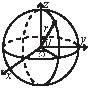
\includegraphics[width=25mm]{../mathematics/sphericalCoordinates}
\end{center}
\[\begin{array}{cc}
x = r\sin\theta\cos\phi & r = \sqrt{x^2+y^2+z^2}\\
y = r\sin\theta\sin\phi & \theta = \textrm{acos}(z/\sqrt{x^2+y^2+z^2})\\
z = r\cos\theta & \phi = \textrm{atan2}(y,x)
\end{array}\]

\section{Derivatives/Integrals}
\begin{align*}
	\dfrac{d}{dx}\arcsin x = \dfrac{1}{\sqrt{1-x^2}} &&& \dfrac{d}{dx}\arccos x = -\dfrac{1}{\sqrt{1-x^2}} \\
	\dfrac{d}{dx}\tan x = 1+\tan^2 x &&& \dfrac{d}{dx}\arctan x = \dfrac{1}{1+x^2} \\
	\int\tan ax = -\dfrac{\ln|\cos ax|}{a} &&& \int x\sin ax = \dfrac{\sin ax-ax \cos ax}{a^2} \\
	\int e^{-x^2} = \frac{\sqrt \pi}{2} \text{erf}(x) &&& \int xe^{ax}dx = \frac{e^{ax}}{a^2}(ax-1)
\end{align*}

Integration by parts:
\[\int_a^bf(x)g(x)dx = [F(x)g(x)]_a^b-\int_a^bF(x)g'(x)dx\]

\section{Sums}
\[ c^a + c^{a+1} + \dots + c^{b} = \frac{c^{b+1} - c^a}{c-1}, c \neq 1 \]
\begin{align*}
	1 + 2 + 3 + \dots + n &= \frac{n(n+1)}{2} \\
	1^2 + 2^2 + 3^2 + \dots + n^2 &= \frac{n(2n+1)(n+1)}{6} \\
	1^3 + 2^3 + 3^3 + \dots + n^3 &= \frac{n^2(n+1)^2}{4} \\
	1^4 + 2^4 + 3^4 + \dots + n^4 &= \frac{n(n+1)(2n+1)(3n^2 + 3n - 1)}{30} \\
\end{align*}

\section{Series}
$$e^x = 1+x+\frac{x^2}{2!}+\frac{x^3}{3!}+\dots,\,(-\infty<x<\infty)$$
$$\ln(1+x) = x-\frac{x^2}{2}+\frac{x^3}{3}-\frac{x^4}{4}+\dots,\,(-1<x\leq1)$$
$$\sqrt{1+x} = 1+\frac{x}{2}-\frac{x^2}{8}+\frac{2x^3}{32}-\frac{5x^4}{128}+\dots,\,(-1\leq x\leq1)$$
$$\sin x = x-\frac{x^3}{3!}+\frac{x^5}{5!}-\frac{x^7}{7!}+\dots,\,(-\infty<x<\infty)$$
$$\cos x = 1-\frac{x^2}{2!}+\frac{x^4}{4!}-\frac{x^6}{6!}+\dots,\,(-\infty<x<\infty)$$

\section{Probability theory}
Let $X$ be a discrete random variable with probability $p_X(x)$ of assuming the value $x$. It will then have an expected value (mean) $\mu=\mathbb{E}(X)=\sum_xxp_X(x)$ and variance $\sigma^2=V(X)=\mathbb{E}(X^2)-(\mathbb{E}(X))^2=\sum_x(x-\mathbb{E}(X))^2p_X(x)$ where $\sigma$ is the standard deviation. If $X$ is instead continuous it will have a probability density function $f_X(x)$ and the sums above will instead be integrals with $p_X(x)$ replaced by $f_X(x)$.

Expectation is linear:
\[\mathbb{E}(aX+bY) = a\mathbb{E}(X)+b\mathbb{E}(Y)\]
For independent $X$ and $Y$, \[V(aX+bY) = a^2V(X)+b^2V(Y).\]

\subsection{Discrete distributions}

\subsubsection{Binomial distribution}
The number of successes in $n$ independent yes/no experiments, each which yields success with probability $p$ is $\textrm{Bin}(n,p),\,n=1,2,\dots,\, 0\leq p\leq1$.
\[p(k)=\binom{n}{k}p^k(1-p)^{n-k}\]
\[\mu = np,\,\sigma^2=np(1-p)\]
$\textrm{Bin}(n,p)$ is approximately $\textrm{Po}(np)$ for small $p$.

\subsubsection{First success distribution}
The number of trials needed to get the first success in independent yes/no experiments, each wich yields success with probability $p$ is $\textrm{Fs}(p),\,0\leq p\leq1$.
\[p(k)=p(1-p)^{k-1},\,k=1,2,\dots\]
\[\mu = \frac1p,\,\sigma^2=\frac{1-p}{p^2}\]

\subsubsection{Poisson distribution}
The number of events occurring in a fixed period of time $t$ if these events occur with a known average rate $\kappa$ and independently of the time since the last event is $\textrm{Po}(\lambda),\,\lambda=t\kappa$.
\[p(k)=e^{-\lambda}\frac{\lambda^k}{k!}, k=0,1,2,\dots\]
\[\mu=\lambda,\,\sigma^2=\lambda\]

\subsection{Continuous distributions}

\subsubsection{Uniform distribution}
If the probability density function is constant between $a$ and $b$ and 0 elsewhere it is $\textrm{U}(a,b),\,a<b$.
\[f(x) = \left\{
\begin{array}{cl}
\frac{1}{b-a} & a<x<b\\
0 & \textrm{otherwise}
\end{array}\right.\]
\[\mu=\frac{a+b}{2},\,\sigma^2=\frac{(b-a)^2}{12}\]

\subsubsection{Exponential distribution}
The time between events in a Poisson process is $\textrm{Exp}(\lambda),\,\lambda>0$.
\[f(x) = \left\{
\begin{array}{cl}
\lambda e^{-\lambda x} & x\geq0\\
0 & x<0
\end{array}\right.\]
\[\mu=\frac{1}{\lambda},\,\sigma^2=\frac{1}{\lambda^2}\]

\subsubsection{Normal distribution}
Most real random values with mean $\mu$ and variance $\sigma^2$ are well described by $\mathcal{N}(\mu,\sigma^2),\,\sigma>0$.
\[ f(x) = \frac{1}{\sqrt{2\pi\sigma^2}}e^{-\frac{(x-\mu)^2}{2\sigma^2}} \]
If $X_1 \sim \mathcal{N}(\mu_1,\sigma_1^2)$ and $X_2 \sim \mathcal{N}(\mu_2,\sigma_2^2)$ then
\[ aX_1 + bX_2 + c \sim \mathcal{N}(\mu_1+\mu_2+c,a^2\sigma_1^2+b^2\sigma_2^2) \]

\section{Markov chains}
A \emph{Markov chain} is a discrete random process with the property that the next state depends only on the current state.
Let $X_1,X_2,\ldots$ be a sequence of random variables generated by the Markov process.
Then there is a transition matrix $\mathbf{P} = (p_{ij})$, with $p_{ij} = \Pr(X_n = i | X_{n-1} = j)$,
and $\mathbf{p}^{(n)} = \mathbf P^n \mathbf p^{(0)}$ is the probability distribution for $X_n$ (i.e., $p^{(n)}_i = \Pr(X_n = i)$),
where $\mathbf{p}^{(0)}$ is the initial distribution.

% \subsubsection{Stationary distribution}
$\mathbf{\pi}$ is a stationary distribution if $\mathbf{\pi} = \mathbf{\pi P}$.
If the Markov chain is \emph{irreducible} (it is possible to get to any state from any state),
then $\pi_i = \frac{1}{\mathbb{E}(T_i)}$ where $\mathbb{E}(T_i)$  is the expected time between two visits in state $i$.
$\pi_j/\pi_i$ is the expected number of visits in state $j$ between two visits in state $i$.

For a connected, undirected and non-bipartite graph, where the transition probability is uniform among all neighbors, $\pi_i$ is proportional to node $i$'s degree.

% \subsubsection{Ergodicity}
A Markov chain is \emph{ergodic} if the asymptotic distribution is independent of the initial distribution.
A finite Markov chain is ergodic iff it is irreducible and \emph{aperiodic} (i.e., the gcd of cycle lengths is 1).
$\lim_{k\rightarrow\infty}\mathbf{P}^k = \mathbf{1}\pi$.

% \subsubsection{Absorption}
A Markov chain is an A-chain if the states can be partitioned into two sets $\mathbf{A}$ and $\mathbf{G}$, such that all states in $\mathbf{A}$ are absorbing ($p_{ii}=1$), and all states in $\mathbf{G}$ leads to an absorbing state in $\mathbf{A}$.
The probability for absorption in state $i\in\mathbf{A}$, when the initial state is $j$, is $a_{ij} = p_{ij}+\sum_{k\in\mathbf{G}} a_{ik}p_{kj}$.
The expected time until absorption, when the initial state is $i$, is $t_i = 1+\sum_{k\in\mathbf{G}}p_{ki}t_k$.

\end{multicols*}
\end{document}